\documentclass[10pt]{article}
\usepackage[paperwidth=39cm, paperheight=39cm, margin=1cm]{geometry}
% Usuń numerację stron.
\pagestyle{empty}

\usepackage{tikz}
% Import do ustalania końcówek strzałek.
\usetikzlibrary{arrows.meta}

% Zmniejsz interlinię.
\linespread{0.9}

% Importy do białych konturów napisów.
\usepackage[T1]{fontenc}
\usepackage{pslatex}
\usepackage{contour}
\usepackage{color}
\contourlength{1pt} % Grubość konturu
\contournumber{50}  % Liczba powtórzeń

% Ustaw czcionkę bezszeryfową.
\renewcommand{\familydefault}{\sfdefault}

\begin{document}
\begin{figure}[p]
\centering
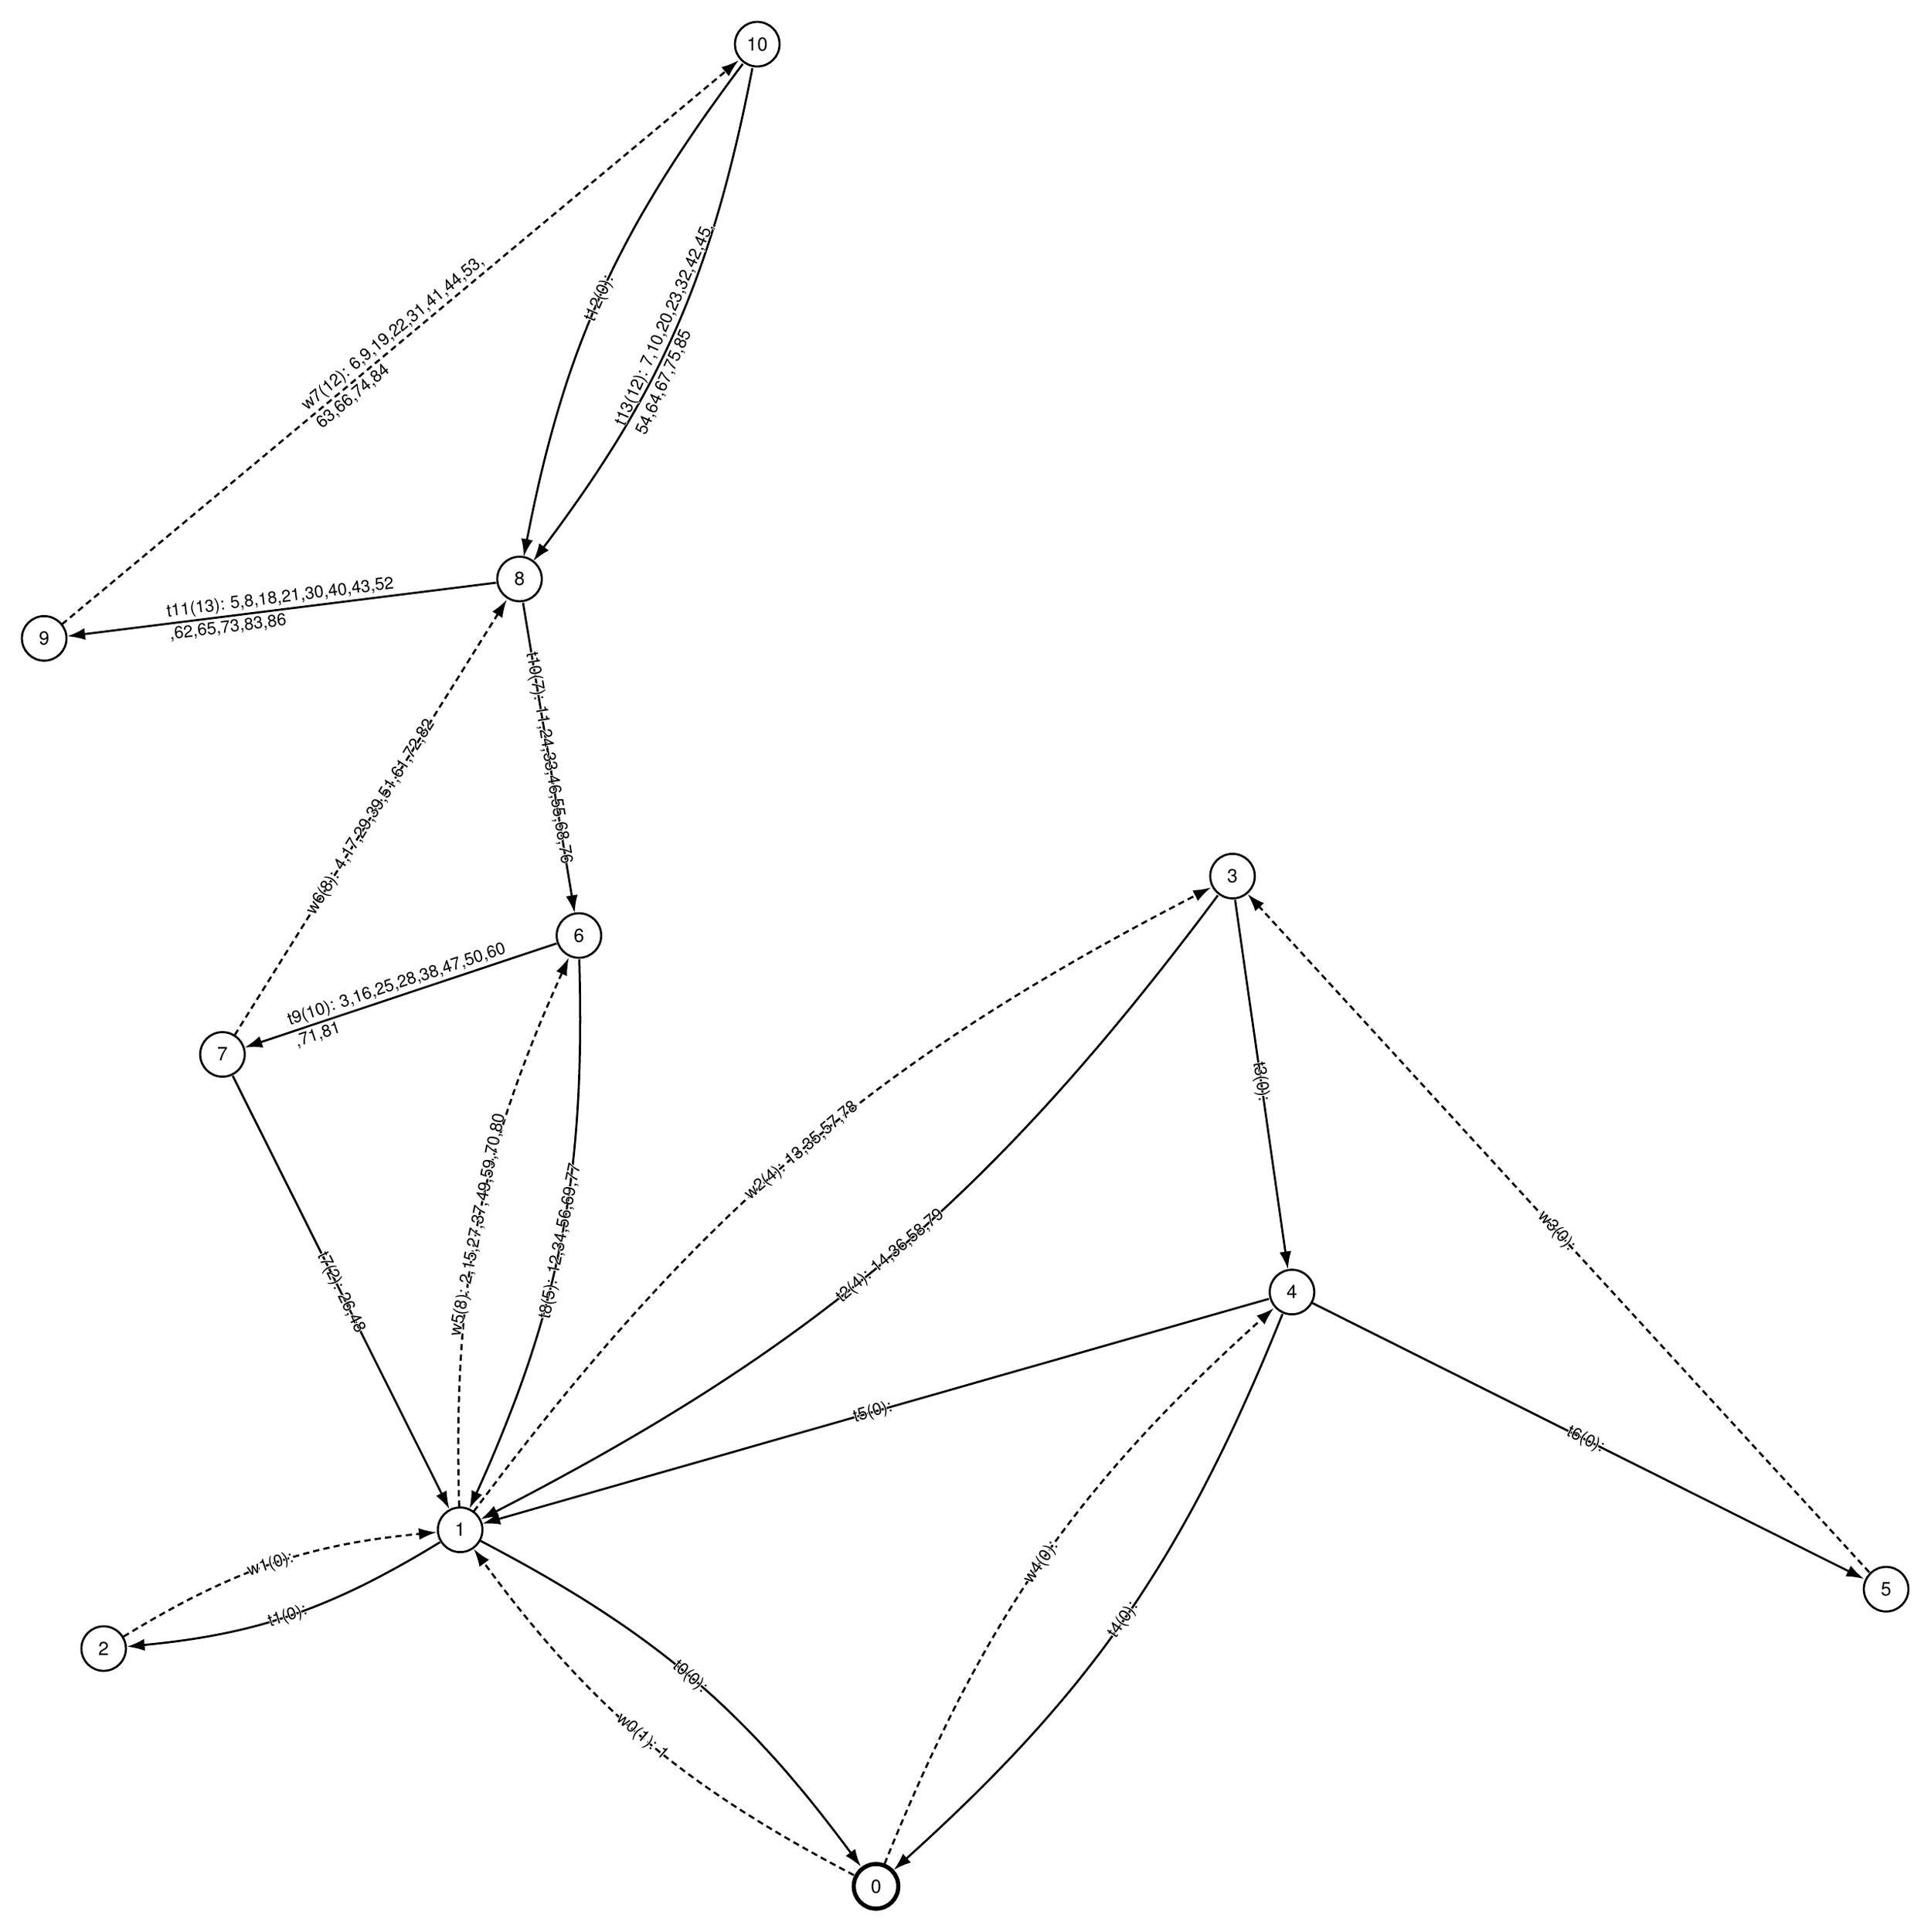
\begin{tikzpicture}[scale=100]
    \tikzset{
        % Style węzłów i krawędzi.
        wezel grafu/.style={circle,draw,minimum size=0.75cm,inner sep=0,line width=0.35mm},
        krawedz grafu/.style={-{Latex[length=3mm, width=2mm]},sloped,centered,line width=0.35mm,font=\small}
    }
    % Węzły:
    \node[wezel grafu,line width=0.7mm] (0) at (16/100, 2/100) {0};
    \node[wezel grafu] (1) at (9/100, 8/100) {1};
    \node[wezel grafu] (2) at (3/100, 6/100) {2};
    \node[wezel grafu] (3) at (22/100, 19/100) {3};
    \node[wezel grafu] (4) at (23/100, 12/100) {4};
    \node[wezel grafu] (5) at (33/100, 7/100) {5};
    \node[wezel grafu] (6) at (11/100, 18/100) {6};
    \node[wezel grafu] (7) at (5/100, 16/100) {7};
    \node[wezel grafu] (8) at (10/100, 24/100) {8};
    \node[wezel grafu] (9) at (2/100, 23/100) {9};
    \node[wezel grafu] (10) at (14/100, 33/100) {10};
    % Krawedzie:
    \path[draw]
    (0) edge[krawedz grafu, bend left=13, densely dashed] node {
        \begin{tabular}{l}
            \contour{white}{w0(1): 1}
        \end{tabular}
    } (1)
    (1) edge[krawedz grafu, bend left=13] node {
        \begin{tabular}{l}
            \contour{white}{t0(0): }
        \end{tabular}
    } (0)
    (0) edge[krawedz grafu, bend left=13, densely dashed] node {
        \begin{tabular}{l}
            \contour{white}{w4(0): }
        \end{tabular}
    } (4)
    (4) edge[krawedz grafu, bend left=13] node {
        \begin{tabular}{l}
            \contour{white}{t4(0): }
        \end{tabular}
    } (0)
    (1) edge[krawedz grafu, bend left=13] node {
        \begin{tabular}{l}
            \contour{white}{t1(0): }
        \end{tabular}
    } (2)
    (2) edge[krawedz grafu, bend left=13, densely dashed] node {
        \begin{tabular}{l}
            \contour{white}{w1(0): }
        \end{tabular}
    } (1)
    (1) edge[krawedz grafu, bend left=13, densely dashed] node {
        \begin{tabular}{l}
            \contour{white}{w2(4): 13,35,57,78}
        \end{tabular}
    } (3)
    (3) edge[krawedz grafu, bend left=13] node {
        \begin{tabular}{l}
            \contour{white}{t2(4): 14,36,58,79}
        \end{tabular}
    } (1)
    (4) edge[krawedz grafu] node {
        \begin{tabular}{l}
            \contour{white}{t5(0): }
        \end{tabular}
    } (1)
    (1) edge[krawedz grafu, bend left=13, densely dashed] node {
        \begin{tabular}{l}
            \contour{white}{w5(8): 2,15,27,37,49,59,70,80}
        \end{tabular}
    } (6)
    (6) edge[krawedz grafu, bend left=13] node {
        \begin{tabular}{l}
            \contour{white}{t8(5): 12,34,56,69,77}
        \end{tabular}
    } (1)
    (7) edge[krawedz grafu] node {
        \begin{tabular}{l}
            \contour{white}{t7(2): 26,48}
        \end{tabular}
    } (1)
    (3) edge[krawedz grafu] node {
        \begin{tabular}{l}
            \contour{white}{t3(0): }
        \end{tabular}
    } (4)
    (5) edge[krawedz grafu, densely dashed] node {
        \begin{tabular}{l}
            \contour{white}{w3(0): }
        \end{tabular}
    } (3)
    (4) edge[krawedz grafu] node {
        \begin{tabular}{l}
            \contour{white}{t6(0): }
        \end{tabular}
    } (5)
    (6) edge[krawedz grafu] node {
        \begin{tabular}{l}
            \contour{white}{t9(10): 3,16,25,28,38,47,50,60} \\
            \contour{white}{,71,81}
        \end{tabular}
    } (7)
    (8) edge[krawedz grafu] node {
        \begin{tabular}{l}
            \contour{white}{t10(7): 11,24,33,46,55,68,76}
        \end{tabular}
    } (6)
    (7) edge[krawedz grafu, densely dashed] node {
        \begin{tabular}{l}
            \contour{white}{w6(8): 4,17,29,39,51,61,72,82}
        \end{tabular}
    } (8)
    (8) edge[krawedz grafu] node {
        \begin{tabular}{l}
            \contour{white}{t11(13): 5,8,18,21,30,40,43,52} \\
            \contour{white}{,62,65,73,83,86}
        \end{tabular}
    } (9)
    (10) edge[krawedz grafu, bend left=-13] node {
        \begin{tabular}{l}
            \contour{white}{t12(0): }
        \end{tabular}
    } (8)
    (10) edge[krawedz grafu, bend left=13] node {
        \begin{tabular}{l}
            \contour{white}{t13(12): 7,10,20,23,32,42,45,} \\
            \contour{white}{54,64,67,75,85}
        \end{tabular}
    } (8)
    (9) edge[krawedz grafu, densely dashed] node {
        \begin{tabular}{l}
            \contour{white}{w7(12): 6,9,19,22,31,41,44,53,} \\
            \contour{white}{63,66,74,84}
        \end{tabular}
    } (10)
    ;
\end{tikzpicture}

\end{figure}
\end{document}
